% Copyright (c) 2026 Islam Ibrahim. All rights reserved.

\documentclass[tikz,border=10pt]{standalone}
\usepackage[T1]{fontenc}
\usepackage{lmodern}
\usepackage{amsmath}
\usepackage{tikz}
\usetikzlibrary{arrows.meta,positioning,calc}

\begin{document}
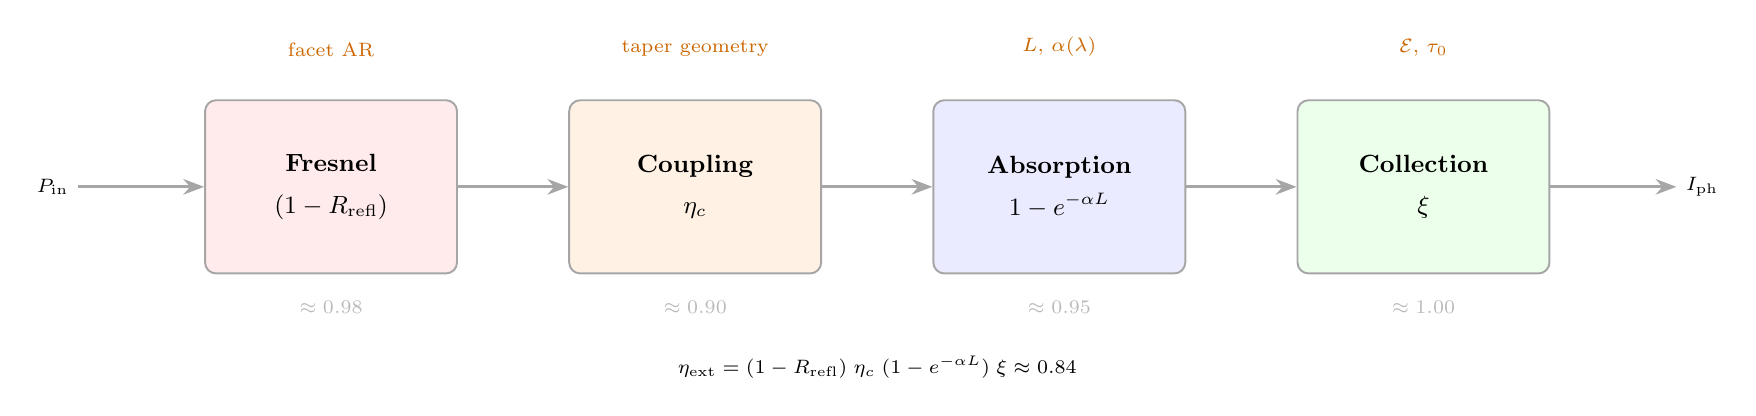
\begin{tikzpicture}[font=\small\rmfamily, >=Stealth,
  lbl/.style={font=\scriptsize\rmfamily},
  stage/.style={draw=gray!70, fill=#1, line width=0.7pt,
    rounded corners=4pt, minimum width=3.2cm, minimum height=2.2cm,
    align=center, font=\small\rmfamily, inner sep=8pt},
  arr/.style={line width=1.0pt, ->, gray!70},
  val/.style={font=\scriptsize\rmfamily, below=6pt, gray!55},
]

%% Input power
\node[lbl] (pin) at (-2.2, 0) {$P_\mathrm{in}$};

%% Stage 1 — Fresnel reflection
\node[stage=red!8, right=16mm of pin] (s1) {%
  \textbf{Fresnel}\\[4pt]
  $(1-R_\mathrm{refl})$};
\node[val] at (s1.south) {$\approx 0.98$};

%% Stage 2 — Optical coupling
\node[stage=orange!10, right=14mm of s1] (s2) {%
  \textbf{Coupling}\\[4pt]
  $\eta_c$};
\node[val] at (s2.south) {$\approx 0.90$};

%% Stage 3 — Absorption completeness
\node[stage=blue!8, right=14mm of s2] (s3) {%
  \textbf{Absorption}\\[4pt]
  $1-e^{-\alpha L}$};
\node[val] at (s3.south) {$\approx 0.95$};

%% Stage 4 — Carrier collection
\node[stage=green!8, right=14mm of s3] (s4) {%
  \textbf{Collection}\\[4pt]
  $\xi$};
\node[val] at (s4.south) {$\approx 1.00$};

%% Output
\node[lbl, right=16mm of s4] (iph) {$I_\mathrm{ph}$};

%% Arrows
\draw[arr] (pin.east) -- (s1.west);
\draw[arr] (s1.east) -- (s2.west);
\draw[arr] (s2.east) -- (s3.west);
\draw[arr] (s3.east) -- (s4.west);
\draw[arr] (s4.east) -- (iph.west);

%% Design lever annotations (above each stage, with more clearance)
\node[lbl, orange!80!black, above=12pt] at (s1.north) {facet AR};
\node[lbl, orange!80!black, above=12pt] at (s2.north) {taper geometry};
\node[lbl, orange!80!black, above=12pt] at (s3.north) {$L$, $\alpha(\lambda)$};
\node[lbl, orange!80!black, above=12pt] at (s4.north) {$\mathcal{E}$, $\tau_0$};

%% Overall EQE result
\node[lbl, align=center, below=26pt] at ($(s2.south)!0.5!(s3.south)$) {%
  $\eta_\mathrm{ext} = (1-R_\mathrm{refl})\;\eta_c\;
  (1-e^{-\alpha L})\;\xi \approx 0.84$};

\end{tikzpicture}
\end{document}
